\documentclass[conference]{IEEEtran}

\usepackage{graphicx}
\usepackage{subfigure}

\usepackage{ifpdf}
\ifpdf
\setlength{\pdfpagewidth}{8.5in}
\setlength{\pdfpageheight}{11in}
\else
\fi

\begin{document}

\title{EMD + sensor data}

% \numberofauthors{2}
% \author{
% % 1st. author
% \alignauthor
% Romain Fontugne\\
%        \affaddr{The University of Tokyo / JFLI, CNRS}
% % 2nd. author
% \alignauthor
% Jorge Ortiz\\
%        \affaddr{University of California, Berkeley}
% \and  % use '\and' if you need 'another row' of author names
% % 3rd. author
% \alignauthor
% David Culler\\
%        \affaddr{University of California, Berkeley}
% % 4th. author
% \alignauthor 
% Hiroshi Esaki\\
%        \affaddr{The University of Tokyo}
% }

\author{\IEEEauthorblockN{Romain Fontugne}
\IEEEauthorblockA{University of Tokyo / JFLI, CNRS}
\and
\IEEEauthorblockN{Jorge Ortiz, David Culler}
\IEEEauthorblockA{Computer Science Division\\
University of California, Berkeley}
\and
% \IEEEauthorblockN{David Culler}
% \IEEEauthorblockA{
% Unversity of California, Berkeley}
% \and
\IEEEauthorblockN{Hiroshi Esaki}
\IEEEauthorblockA{University of Tokyo}
}



\maketitle

% % A category with the (minimum) three required fields
% \category{H.4}{Information Systems Applications}{Miscellaneous}
% %A category including the fourth, optional field follows...
% \category{D.2.8}{Software Engineering}{Metrics}[complexity measures, performance measures]
% 
% \terms{Delphi theory}
% 
% \keywords{ACM proceedings, \LaTeX, text tagging}

% (This is included by thesis.tex; you do not latex it by itself.)

\begin{abstract}

% The text of the abstract goes here.  If you need to use a \section
% command you will need to use \section*, \subsection*, etc. so that
% you don't get any numbering.  You probably won't be using any of
% these commands in the abstract anyway.

% Invasive brag; forbearance.



This thesis examines the state of the art of building information systems and evaluates their architecture in the context
of emerging technologies and applications for deep analysis of the built environment.  
We observe that modern building information systems are difficult to extend, do not provide general services for application development, do not
scale, and are difficult to set up and manage. 
We assert that a new architecture must be designed with four system properties -- \emph{extensibility, generalizability, scalability,
ease of management} -- in order to address these shortcomings.  
Our system, StreamFS, embodies these system properties through a filesystem abstraction and a set of data services.
% We propose a new architecture that embodies these system principles through a filesystem abstraction and data services, called StreamFS.  
Data services are made available to applications through an overloaded pipe abstraction.  This allows for dataflow specification
of processing streams to clean and analyze the streaming sensor data.

We deploy StreamFS in seven different buildings and compose several applications on top of it.  One of the driving
applications is a phone application called the Mobile Energy Lens.  The Energy Lens provides occupants with mechanisms for 
collecting building information
in a unified platform and provides a way to view aggregate energy consumption data associated with the spatial deployment configuration 
of plug-load devices.  We present a three-layer architecture, where one of the main layers is implemented entirely with 
the data management and processing services offered by StreamFS.  

We introduce the notion of verification of physical relationships through empiricial data.  
We partition the verification problem into three sub problems: 1) functional verification, 2) spatial verification, and 3) categorical
verification.  We show how empirical mode decomposition, correlation, and standard machine learning techniques can give us 
information about how the sensors are related to each other, statistically and physically.
We demonstate an \emph{extensible, generalizable, scalable, and easy-to-manage} system for supporting the ``appification'' of the 
built environment.  


% We examine the 
\end{abstract}

\subsection{Introduction}
Buildings consume an enormous amount of energy in countries around the world.  In 
Japan, 28\% of the energy produced is consumed in buildings~\cite{japanbuildings} while in the United 
States it is as high as 40\%~\cite{epabuildings}.  Moreover, studies show that between 30-80\% of it
is wasted~\cite{waste_science, next10_waste}.  Large commercial buildings are typically instrumented
with a large number of sensors measuring various aspects of building operation.  Although this data is
typically used to assure operational stability, they may also be used to measure, observe, and identify
instances of wasted use.

Identifying instances of wasted energy use is non-trivial.  System efficiency is defined as the ratio of the 
useful work done to the energy it consumes.  In the case of buildings, we broadly define useful work as 
the energy used to support occupant activities.  From the perspective of the building that means maintaining
a comfortable temperature setting, providing power for plug-load devices, and providing adequate lighting
conditions; particularly in spaces that are occupied.  However, identifying efficient use of resources,
\emph{especially} when a space is occupied, is difficult.  Typically it involves deep knowledge of the usage scenario and
a meaningful understanding of what it takes to support the activity.  Furthermore, situations and activities differ
greatly.  The outside weather changes, varying schedules affect occupancy, rooms have lectures, class,
or other office activities.  Simply put, the process is time consuming, requires specialized knowledge,
and does not scale.

Devices are typically used together in some fashion.  For example, in an office
setting a person enters their office, turns on their PC and lights, etc.
When the person leaves the office, they revert back to the state their devices were in before arrival.
If one of the items is not reverted to its pre-arrival state, waste occurs. 
%Waste occurs when something is left on.
The same is true about equipment usage.  When the outside temperature is low the heater turns on.
% and
%the negation is also true.  If the temperature is high and the heater is on, waste occurs.  
\emph{Waste occurs when abnormal in-concert usage patterns arise}.  
%For example, 
% Moreover, if the heating and cooling system are on 
% simultaneously~\cite{simheatcool}, that is a problem that is \emph{particularly} wasteful and hard to 
% detect by occupants.  
Fundamentally, understanding ``normal'' spatio-temporal usage patterns between devices could help
identify problems when devices are not being used correctly.
We conjecture that inefficient energy use can be identified through anomalies in the correlation
patterns between devices.  We examine device correlation patterns in this paper and look specifically
at processing raw sensor traces, such that the correlations we find are meaningful.

In this paper, we present early results for correlating usage patterns across a large number of sensors
in a single deployment.  We analyze data from a 12-story office building at the University of Tokyo.  
The deployment consists of almost 700 sensors monitoring a broad range of devices inside and outside 
the building.  Our initial observations and results include the following:

\begin{enumerate}
\item Raw-trace correlation analysis is too strongly influenced by the common low-frequency trends in the data
	to identify meaningful relationships.
\item Using a technique called empirical model decomposition (EMD)~\cite{huang:emd1998} removes this 
		 trend and helps identify truly correlated sensor traces.
\item We can construct clusters of correlated sensors that are spatio-temporally correlated, \emph{without
		a priori knowledge of their placement}.
\end{enumerate}

In the rest of the paper we explain EMD and how we use it, we show various examples of our technique on real-world
traces, and we discuss the implications and future work.

% Green IT

% Understand the energy consumption of a building and identify savings opportunities.

% Identification of energy consuming devices that are correlated.
% Uncover usage patterns of correlated device that are energy efficient.
% Detect deviation from the energy efficient pattern and report to the user.

% During the design of our application the first difficulty was to identify the set of devices that have related energy consumption.

% This article focuses on this problem.

% Results:
% \begin{enumerate}
% \item Correlation is noisy and can't find inter-relationships between sensors
% 		with subtle differences.
% \item Underlying behavior should extract most-common denominator in comparing traces
% 		to observe truly correlated behavior.
% \item Empirical mode decomposition (EMD) can be used to compare underlying behavior after the
% 		removal of the dominant frequencies in the signal.
% \end{enumerate}

% \subsection{ideas}

% Future work:
% \begin{enumerate}
% \item We can create a time-varying dependency graph to compare ``normal'' versus ``abnormal'' behavioral
% 		patterns in underlying use.
% \item We can codify ``normal'' or ``efficient'' graphs and compare with real graph constructs over time.
% \end{enumerate}

% Possible algorithms:
% \begin{enumerate}
% \item find correlated and uncorrelated sensors
% \item construct correlation network where the nodes are the sensors and an edge implies correlation above
% 		threshold. (We can also construct the complement of that.)
% \end{enumerate}


\subsection{Dataset}
The data we used was obtained from a deployment of sensors in a 12-story office building
on the campus of the University of Tokyo~\cite{gutp, ogawa:lncs2011}.  The deployment consists of 
almost 700 sensors monitoring device power consumption, ranging from plug-load devices to components of the
heating, ventilation, and air conditioning system (HVAC) and lighting.  Sensors also reported temperature, 
pressure, device-state, and other information.  Each sensor reports data on the
order of minutes.  Over 500 GBs of data was collected over a 2-year span.

\begin{figure*}[tb]
\hspace{-2cm}
\includegraphics[width=1.2\textwidth]{figs/emd_25_26-eps-converted-to}
\vspace{-1cm}
\caption{Decomposition of the EHP and light trace using bivariate EMD. IMFs correlation coefficients highlight the intrinsic relationship of the two traces.}
\label{fig:emd}
\end{figure*}

% The intent of the Green University of Tokyo Project (GUTP) \cite{gutp} is to reduce the university environmental impacts associated to its electric energy consumption.
% The first step of this project was to deploy sensors at the Building No.2 of the Faculty of Engineering 
% Electric power consumption of a 12 floors building containing researchers office and classroom.
% 1215 sensors monitoring different devices...

%received attention in the past \cite{ogawa:lncs2011}.

For this investigation, we focus on a three-week span in the summer of 2011 (from July 4th to July 24th).
The dataset captures regular work days, weekends, and one holiday (July 18th).  This timeframe captures
the typical usage of the equipment, triggered by occupant activity.  For the initial
analysis, we focus on three sensors; two water pumps and a light feed.  The first pump is an 
``electric heat pump'' and is labled as EHP, the second  is a ``gas heat pump''
and labeled as GHP.  The room lighting system serves the same room as the EHP.  The GHP
serves a different room on the same floor.  The expanded portion of our analysis pivots around the EHP
and does a pairwise comparison between it and all other sensors in the building.
Computationally, this approach does not scale to a large number of sensors.  For future work, we will
examine various heuristics to narrow the search space before running pairwise comparisons.

% includes one day holiday (July 18th)
% 3 different sensors:
% \begin{itemize}
%  \item Two are measuring the electric power consumption of two devices from the same room; an electric heat 
%  		pump (EHP) and the room lighting system.
%  \item One is measuring the electric power consumption of a gas heat pump (GHP) that is pumping water to cool 
%  		a different room in the same building.
% \end{itemize}

% Later we expand our analysis to include all the sensors in the building.


\subsection{Problem statement and Initial approach}\label{problem}
% In our analysis, we are focused on finding devices that are correlated in their use over time.  Therefore, the
% main objective is to examine how device traces relate to one another.  The wish to identify
% correlated device-trace patterns at large spatio-temporal scales.

In buildings, metadata is poorly and unsystematically managed within a single system domain.  Moreover, 
with the ever growing number of additional sub-meters, it is important to quickly integrate
sensor data from multiple systems to understand the full state of the building.  It is also important to 
understand how sensors are used in concert.  Anomalies in usage may indicate underlying problems with 
the equipment or inefficient/incorrect usage.  

Figure \ref{fig:raw} shows the raw traces for the three devices discussed in 
the previous section (EHP, GHP, light). All three exhibit a diurnal usage pattern.  On weekends, each
draw less power.   For our initial analysis, we calculated the pairwise 
correlation coefficient for all sensors in the set.  The correlation coefficient for 
 the EHP and light is $0.7715$ and the correlation coefficient for the EHP and GHP is $0.6370$.
Running correlation across them yields high correlation coefficients, mostly
due to their underlying daily usage pattern.


% \begin{figure}[t!]
% \centering
%  \subfigure[EHP trace]{\label{fig:raw_ehp}\includegraphics[width=.4\textwidth]{img/25.png}}
%  \subfigure[Light trace]{\label{fig:raw_light}\includegraphics[width=.4\textwidth]{img/26.png}}
%  \subfigure[GHP trace]{\label{fig:raw_ghp}\includegraphics[width=.4\textwidth]{img/41.png}}
%  \caption{Traces from three different sensors captured in 2011 from July 4th to July 24th. Data is normalized and aggregated into 30 minutes time bins.}
%  \label{fig:raw}
% \end{figure}


Our initial results were not surprising.  The diurnal pattern dominates the comparison between the sensors.
Weather is the main driver for this behavior and it affects the readings in almost all of the
sensors in our dataset.  Cross-correlation on raw sensor data is insufficient for filtering intrinsically related
behavior.  Upon closer examination of the data we assess the following:

\begin{itemize}
\item The main underlying diurnal trend occurs in almost all the traces.
\item Occupancy and room activities occur at random times during the day and change 
		at a higher frequency than weather patterns.
\item Sensors that serve the same location observe the same activities.  Therefore, their underlying
		measurements should be correlated.
\end{itemize}

In order to uncover these relationships we must remove low-frequency trends in the traces and
compare the readings at high frequencies.

% \begin{table}
% \begin{center}
% \begin{tabular}{|l|l|l|l|l|l|}
% \hline
% × & Raw trace & 1st IMF & 2nd IMF & 3rd IMF & Residual\\ \hline
% EHP, Light & 0.7715 & 0.43909 & 0.49344 & 0.63469 & 0.82132 \\ \hline
% EHP, GHP & 0.6370 & 0.0060274 & 0.063546 & 0.16764 & 0.79378 \\ \hline
% \end{tabular}
% \caption{Correlation coefficients of the analyzed trace and their IMFs uncovered by EMD}
% \label{tab:corr}
% \end{center}
% \end{table}
% \subsection{Simple Scenario}

\begin{figure*}[tb]
\hspace{-2cm}
\includegraphics[width=1.2\textwidth]{figs/emd_25_41-eps-converted-to}
\vspace{-1cm}
\caption{Decomposition of the EHP and GHP trace using bivariate EMD. IMFs correlation coefficients highlight the intrinsic independence of the two traces.}
\label{fig:emd2}
\end{figure*}

% The small difference between the two computed correlation coefficients is misleading as one could conclude that the three signals are correlated and the corresponding devices are activated by a single action.

% The high correlation coefficients obtained for these three signals result .... weekly pattern....
% small difference = local fluctuation...

% this high score comes from the fact that the two devices are monitoring offices that are weekly used.

% Indeed the weekly pattern of the data trump the correlation coefficients....

% How to inspect only the local fluctuations...?
% we'd like to have an elegant solution (i.e. not specifying the interesting time scale)





\section{Methodology}\label{method}
%Remove the weekly trend of the data to analyze the detailed changes that convey the device behavior at small time scales.

% Our initial approach examined correlation analysis on raw sensor traces.  However, we quickly
% found that correlation is overly sensitive to fluctuations in the data.
Fundamentally, the readings are driven by the same underlying phenomena: 
weather and occupancy.  Weather influences \emph{all} the data similarly.  Occupancy, however, changes
throughout the building and should be used as a differentiating component in the signal
comparisons.  Sensors that share spatio-temporal elements should be correlated after the removal
of the underlying trend driven by the weather.  In order to find unique relationships we need to remove 
this common trend.

\subsection{Empirical Mode Decomposition}
Empirical Mode Decomposition (EMD) \cite{huang:emd1998} is a new technique used for de-trending data.
Specifically, EMD detrends non-stationary, non-linear timeseries data.  
% A trend is defined as 
% an intrinsically determined monotonic function within a certain temporal span or a function in which there 
% can be at most one extremum within that temporal span.  
A non-stationary signal is a signal whose mean and
variance change over time.  EMD is a process, not a theoretical tool.  Its main use is for removing trends 
to enable more useful spectral analysis.

We describe the EMD process as follows:  for a signal \emph{X(t)}, let $m_1$ be the mean of its upper and
lower envelopes as determined from a cubic-spline interpolation of local maxima and minima. The locality 
is determined by an arbitrary parameter.

\begin{enumerate}
\item The first component $h_1$ is computed: $h_1=X(t)-m_1$
\item In the second sifting process, $h_1$ is treated as the data, and $m_{11}$ is the mean of $h_1$'s upper and lower envelopes: $h_{11}=h_1-m_{11}$
\item The procedure is repeated $k$ times, until $h_{1k}$ is a function: $h_{1(k-1)}-m_{1k}=h_{1k}$
\item Then it is designated as $c_1=h_{1k}$, the first functional component from the data, which contains the shortest period component of the signal. We separate it from the rest of the data: $X(t)-c_1 = r_1$, and the procedure is
repeated on $r_j: r_1-c_2 = r_2,\dots,r_{n-1} - c_n = r_n$
\end{enumerate}

The result is a set of functions called intrinsic mode functions (IMF); the number of functions in 
the set depends on the original signal~\cite{emd_process}.  An IMF is any 
function with the same number of extrema and zero crossings, with its envelopes being symmetric with respect to zero.
We run our correlation analysis on the shared IMF outputs between a pairs of signals.  In order to ensure 
that the IMFs corresponding to two distinct signals are on the same time scale, we use 
bivariate EMD \cite{rilling:biemd2007} to decompose two signals at once. 

\section{Results}
This section emphasize the advantages of EMD to efectively uncover correlated signals/sensors(?).
First, we demonstrate the benefit of EMD with a simple example, the three sensorsr presented in Section \ref{problem}.
Second, we validate the proposed methodology with a large dataset (674 sensors) and highlight that EMD uncovers the spatial correlation of the sensors.

\begin{table*}
\begin{center}
\begin{tabular}{|l|l|l|l|l|l|}
\hline
× & Raw signal & 1st IMF & 2nd IMF & 3rd IMF & Residual\\ \hline
EHP, Light & 0.7720 & 0.4431 & 0.5104 & 0.6171 & 0.8114\\ \hline
EHP, GHP & 0.6369 & -0.0055 & 0.0883 & 0.2350 & 0.7956\\ \hline
\end{tabular}
\caption{Correlation coefficients of the analyzed signal and their IMFs uncovered by EMD}
\label{tab:corr}
\end{center}
\end{table*}
\subsection{Simple Scenario}

Lets consider the simple example of Section \ref{problem} where we would like to know if an EHP signal is correlated with the two other signals; a light signal and a GHP signal.
Using the raw signals, the correlation coefficients suggest that the light and GHP signals are both correlated to the EHP signal (Table \ref{tab:corr}).
As stated in previous section this result is certainly biased by the strong daily pattern shared by these three signals.

Extracting the weekly pattern of the data using EMD permits a more detailed analysis of these signals.
Figure \ref{fig:emd} depicts the EMD decomposition of the three signals.
Notice that the EMD process has been stopped once the daily pattern have been uncovered.
Thereby, for each signal EMD has retrieved three IMFs that highlight the high frequency characteristics of the signals.

The correlation coefficients for the EHP and light IMFs --- i.e. $0.4431$, $0.5104$ and $0.6171$ corresponding respectively to the IMF1, IMF2 and IMF3 --- emphasize the positive correlation of the two signals in the high frequency domain.
However, the correlation coefficients for the EHP and GHP IMFs show that the two signals are independent in the high frequency domain.
Therefore, EMD allow us to effectively identify that the light signal is related to the EHP whereas the GHP one is not.

\begin{figure*}
\centering
 \subfigure[Raw signals correlation coefficients]{\label{fig:histo1}\includegraphics[width=.45\textwidth]{img/allFloors_week1_week4_corr_abs.eps}}
 \subfigure[Average IMFs correlation coefficients]{\label{fig:histo2}\includegraphics[width=.45\textwidth]{img/allFloors_week1_week4_emd_abs.eps}}
 \caption{Distribution of the correlation coefficients of the raw signals and corresponding IMFs using 3 weeks of data from 674 sensors deployed on 12 Floors.}
\label{fig:histo}
\end{figure*}

\subsection{Validation}


In order to validate the effectiveness of the proposed approach to identify correlated signals, we analyze three week signals from the 674 sensors deployed in the building.
For each signal $S$ we compute the correlation coefficient for $S$ and the EHP signal and the average value of the IMFs correlation coefficients obtained with EMD.
Figure \ref{fig:histo1} shows the distribution of the raw signal correlation coefficients.
Regarding this figure a large fraction of the dataset seems to be correlated with the EHP signal.
Indeed half of the analyzed signals provide a correlation coefficient higher than $0.36$.
Although the highest score correspond to the light signal that is actually from the same room as the EHP signal, all signals that achieve a score higher than $0.6$  correspond to 118 heat pumps that are located at different floors and are independent from the analyzed EHP signal.
Moreover, the distribution of the signals is almost uniform, thus, discriminating signals correlated to the analyzed one is a laborious task.

Figure \ref{fig:histo2} shows the distribution of the average correlation coefficients for the IMFs of each signal and the analyzed EHP one.
Here the number of signals correlated to the analyzed one is significantly small. 
Only 10 signals perform a score higher than $0.25$ and their distribution allow us to easily rank signals in term of correlation.

Interestingly the IMFs correlation coefficients reveal the spatial correlation of the sensors.
Figure \ref{fig:map} is the map floor where the EHP signal is measured.
Specifically, the EHP reports heating activity in the room $C2$.
Regarding the results from the IMFs correlation coefficients, the signal performing the highest score (i.e. $0.522$) is the signal corresponding to the lighting system of the same room.
The two highest scores for this floor (i.e. $0.316$ and $0.279$) are the light and EHP signals from next door, room $C1$.
Lower values correspond to sensors measuring activities in other rooms that have no specific relations with the analyzed signal.
% in the simple scenario the GHP is located in the room A5.

\begin{figure}
\includegraphics[width=.5\textwidth]{img/floorMap.png}
\caption{}
\label{fig:map}
\end{figure}

\section{Future work and conclusion}
In this paper we examined two system challenges -- mobility and consistency management -- for enabling and energy 
analytics applications in buildings.  We also 
offered initial solution approaches.  We
see these as crucial barriers to solve in order to provide the kinds of services described in Section~\ref{sec:vision}.
However, other challenges remain, particularly those related to scaling to an entire buildings, integrating
many more streaming data sources, and providing streaming analytics for immediate display to building occupants.
We see an opportunity to combine these with control in order to empower building occupants to literally take
control of their energy footprint.  The components of our architecture are simple, and simplicity is important for scale and
generalizability.  We hope that with the right tools and information, people will be motivated to act, and large
energy waste reduction can be achieved.


\section*{Acknowledgments}
The authors thanks ....(Patrick, Patrice, Pierre for EMD, Ochiai-san for the data, Kensuke, Young for discussion)
This research was partially supported by the JSPS fellowship program.

\bibliographystyle{abbrv}
\bibliography{references}

\end{document}
